\documentclass[11pt]{article}

\usepackage{rotating}
\usepackage{array}
\usepackage{graphicx}
\usepackage[letterpaper]{geometry}

\newcommand{\twoxtwo}{$2\times2$}
\newcommand{\threexthree}{$3\times3$}

\title{Measuring the Complexity of All the Art}
\author{Jonathan Langke and Peter Boothe}
\date{\today}

\begin{document}
\maketitle

\begin{abstract}
We define formula complexity based on a restriction of Kolmogorov complexity,
and measure the formula complexity of all possible \twoxtwo\ and \threexthree\
artworks.  We have also conducted a survey of the relative perceived visual
complexity of these artworks, and we report that survey's results.  We end by
discussing the links between these two notions, and find that formula
complexity does seem to be related to visual complexity.
\end{abstract}

\section{Introduction}

Art has many definitions, but the one we will use here is that a piece of black
and white digital art is a matrix where every entry is either true or false.
An artwork can be generated from a mathematical formula that evaluates to a
boolean and involves integers $x$ and $y$.  For our initial study, we
considered only \twoxtwo\ matrices, because there are only $2^{2\cdot2} = 16$
of them, and they could therefore be exhaustively generated.

The Kolmogorov Complexity or program-size complexity of a particular object is
the size of the smallest program which outputs that object.  This allows us to
talk about the complexity (and randomness) of individual items.  Kolmogorov
complexity is, unfortunately, uncomputable.  It is, however, recursively
enumerable (RE).  Therefore, we can enumerate all well-typed expressions and
evaluate them on multiple inputs.  The size of the smallest expression which
outputs that object is then its Kolmogorov complexity!

Our algorithm to generate all the art, and keep track of its Kolmogorov
Complexity is as follows: Enumerate all well-typed programs of size 1.  For
each enumerated formula, generate its corresponding artwork.  If this artwork
has not been previously generated, then it has Kolmogorov complexity 1.  Next,
we repeat for size 2, 3, 4, etc., until we have managed to generate all
possible \twoxtwo\ artworks.  To do this, however, we must first define what we
mean by a ``well-typed program''.

A program is well-typed if the inputs types of the functions match the type of
those function's arguments.  An example of an ill-typed program is {\tt (+
false 3)}, whereas a well-typed program is {\tt (+ 3 x)}.  We further require
that the overall type of our program be {\tt (int, int) -> bool}.  An example
of such an expression is {\tt ($\lambda$ (x y) (< x y))}, which is an
expression with two inputs, which evaluates to either true or false.

Further, we also need to define our programming language.  Our language is
constructed out of the atoms {\tt < + * x y 1 0 and or not true false}.


\begin{figure}
\begin{center}
\begin{tabular}{r | p{2in}   p{2in}}
Expression & (x $<$ y) &
(((1 + (1 + 1)) $<$  (x * y)) and 
          ((x + 1) $<$ (y * (1 + 1)))) \\
Expression Size & 3 symbols & 19 symbols\\
  Artwork & 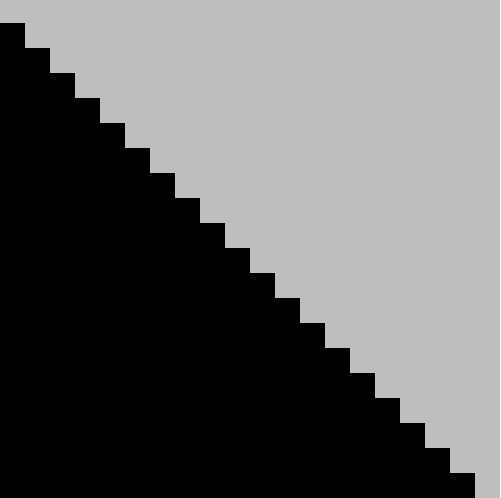
\includegraphics[width=1.5in]{../presentation/simple.png} &
  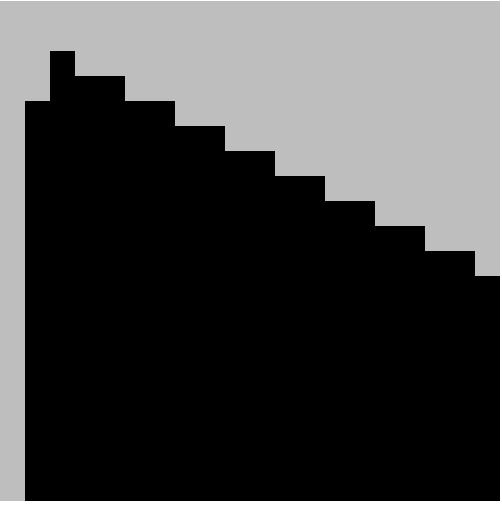
\includegraphics[width=1.5in]{../presentation/complex.png} \\
Kolmogorov Complexity& 3 &
19
\end{tabular}
\end{center}

\caption{Two artworks of differing formula complexity}
\end{figure}



The natural extension of our exploration of all the 2x2 artwork and the structure within the set of 2x2 artwork as a whole is the following question. What is the correlation between visual complexity (an inherently subjective notion) and
Formula complexity?  

\section{Formula Complexity}
Formula complexity is a ``low-powered'' version of Kolmogorov Complexity.  KC
allows the full power of a programming language to be put to bear in describing
how an output is produced.  In particular, KC allows for the definition and
application of functions as well as conditional statements.  In our language,
the only things which can be used are formulae with a boolean result
involving only the logical atoms {\tt and}, {\tt or}, {\tt not}, {\tt true},
and {\tt false}, as well as the numerical atoms of {\tt 0}, {\tt 1}, {\tt x},
{\tt y}, {\tt +}, {\tt *}, and {\tt <}.

Because formula complexity disallows loops and function definitions, every
formula represents a terminating program.  Even more, since the domain of all
of the operators is total, this means that every well-typed formula represents
a non-crashing program\footnote{This is why the division and modulus operators
were excluded, as {\tt 12 mod 0} and {\tt 12 / 0} result in a crashing program
rather than a value.}.  Thus, in exchange for ``powering down'' KC, we can
actually enumerate and test all formulae, without worrying about infinite loops
or crashes.

Each formula evaluates to a boolean and involves the variables $x$ and/or $y$.
Therefore, to create a $3\times3$ artwork from a formula, simply evaluate the formula
at all of the points $(x,y) = (0,0)$, $(x,y) = (0,1)$, $(x,y) = (0,2)$, $(x,y)
= (1,0)$, $\ldots$, and $(x,y) = (2,2)$.  Where the formula evaluates to true,
set the corresponding square on the art to black, and where the formula is
zero, set the square to white.  Every artwork has multiple formula which
produce it.  The formula complexity of an individual artwork is the smallest
such formula.

As an example, the all-black is produced by the formula {\tt true}, {\tt not
false}, {\tt true or false}, and many many others.  However, because the
smallest such formula consists of just one atom, the formula complexity of the
all-black artwork is 1.  From this example (and from the definition), we see
that formula complexity is a property of an artwork, not a formula.  The
formula complexity is defined as the size of the smallest formula able to
produce the output in question. 

\subsection{Generating The Art}

To generate all the art, we first generate all well-typed boolean formulae, in
order of size.  Then, for each formula, we generate its corresponding artwork.
If this is the first time that artwork has been generated, we then know that
the formula complexity of the artwork is equal to the size of the formula just
used.  Generating all the \twoxtwo\ formulae revealed some hidden structure to our
results.

\subsubsection{All the \twoxtwo\ Art}

From Figure~\ref{fig:2x2}, some things are immediately obvious.  First of all,
as might match one's intuition, the all-black and all-white pictures are the
least complex pictures.  Secondly, one can see that if a formula of size $n$
exists to create a certain picture, then that picture's inverse has a
complexity of one of $n-1$, $n$, or $n+1$.  Examples of this last phenomenon
can be seen between levels 7 and 8, as well as between levels 3 and 4.  This occurs
for the simple reason that adding one symbol ({\tt not}) creates a picture's
inverse.  Also, somewhat intriguingly, we can see gaps at 2 and 6.  Although
there are formulae of size 2, none of those formulae produce a picture that has
not been already produced by formulae of a smaller size e.g {\tt (not true)}
and {\tt (not false)} are more succinctly expressed as {\tt false} and {\tt
true}.

Also visible in our results is that if an artwork has formula complexity of
$n$, then the diagonal flip of that artwork also has formula complexity of $n$,
because exchanging $x$ and $y$ results in a formula of exactly the same size.
This can be seen in levels 3, 4, and 5 of Figure~\ref{fig:2x2}.

\begin{figure}
\begin{center}
\begin{tabular}{r c l}
Formulae & Level & Pictures \\
\tiny{none} & 0 & empty \\
\tiny{(true), (false)} & 1 &
    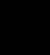
\includegraphics[width=.25in]{../presentation/2x2/Shape1LVL1.png}~
    
\includegraphics[width=.25in]{../presentation/2x2/Shape2LVL1.png} \\
\tiny{none} & 2 & empty \\
\tiny{($<$ x 1), ($<$ y 1), ($<$ x y), ($<$ 0 x), ($<$ 0 y), ($<$ y x)} & 3 & 
    
\includegraphics[width=.25in]{../presentation/2x2/Shape1LVL3.png}~
    
\includegraphics[width=.25in]{../presentation/2x2/Shape2LVL3.png}~
    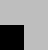
\includegraphics[width=.25in]{../presentation/2x2/Shape5LVL3.png}~
    
\includegraphics[width=.25in]{../presentation/2x2/Shape6LVL3.png}~
    
\includegraphics[width=.25in]{../presentation/2x2/Shape3LVL3.png}~
    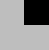
\includegraphics[width=.25in]{../presentation/2x2/Shape4LVL3.png}\\
\tiny{(not ($<$ x y)), (not ($<$ y x))} & 4 & 
    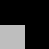
\includegraphics[width=.25in]{../presentation/2x2/Shape2LVL4.png}~
    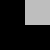
\includegraphics[width=.25in]{../presentation/2x2/Shape1LVL4.png} \\
\tiny{($<$ (y + x) 1), ($<$ (y * x) 1), ($<$ 0 (y + x)), ($<$ 1 (y + x))} & 5 & 
    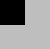
\includegraphics[width=.25in]{../presentation/2x2/Shape2LVL5.png}~
    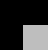
\includegraphics[width=.25in]{../presentation/2x2/Shape1LVL5.png}~
    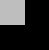
\includegraphics[width=.25in]{../presentation/2x2/Shape3LVL5.png}~
    
\includegraphics[width=.25in]{../presentation/2x2/Shape4LVL5.png} \\
\tiny{none} & 6 & empty \\
\tiny{(or ($<$ y  x) ($<$ x  y))} & 7 &
    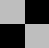
\includegraphics[width=.25in]{../presentation/2x2/Shape1LVL7.png}\\
\tiny{(not (or ($<$ y  x) ($<$ x  y)))} & 8 &
    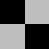
\includegraphics[width=.25in]{../presentation/2x2/Shape1LVL8.png}
\end{tabular}
\end{center}

\caption{All the \twoxtwo\ art with its corresponding complexity.}
\label{fig:2x2}
\end{figure}

After generating all \twoxtwo\ artworks, we found that the artworks were too
small for people to feel comfortable discussing those artworks' visual
complexity.  Therefore, we set our sights higher.

\subsubsection{All the \threexthree\ Art}

Generating all of the \threexthree\ art proved to be a more significant
computational challenge.  Even with some rudimentary pruning, we still had tens
of billions of formulae to check.  Our preliminary results may be seen in
Figure~\ref{fig:3x3}.  Note that although there were no new artworks in level 6
in the \twoxtwo\ results, there are new artworks at that level in the
\threexthree\ artworks --- these new artworks differ from smaller ones only in
their last column or row, and so these differences were not relevant to the
\twoxtwo\ case.

\begin{figure}
\begin{center}
\begin{sideways}
\input{3x3table.tex}
\end{sideways}
\end{center}

\caption{All the \threexthree\ art with its corresponding complexity.}
\label{fig:3x3}
\end{figure}

After generating all the \threexthree\ artworks, we wished to discover whether
our notion of formula complexity had anything to do with visual complexity.


\section{Assessing Visual Complexity}

There is an intuitive notion of ``visual complexity'', but it is unclear
whether any two people would agree on whether a particular artwork is visually
complex. It is also not known whether visual complexity is related to
computational complexity.  In an effort to discover whether visual complexity
is something that people agree upon, and to discover whether formula complexity
is related to perceived visual complexity, we conducted a survey via a website.

We constructed two websites that asked visitors to choose which of two images
they found to be of greater visual complexity.  One website asked about all the
\twoxtwo\ art, and the other asked about all of the \threexthree\ art.  Both
such sizes are small enough to completely enumerate (there are 16 and 512
artworks in each respective category) as well as small enough to calculate the
formula complexity of each artwork.

We then asked users on Twitter as well as local campus students to repeatedly
assess which of two images they found more visually complex.  We treated each
assessment as if it were a competition between two players (artwork one vs
artwork two), and when the user decided upon a winner, we used the
TrueSkill\texttrademark\ algorithm to update each artwork's relative visual
complexity based on each match's results.


\section{Combined Results}

% a scatterplot of "measured visual complexity" vs "formula complexity"
Scatterplot goes here along with more discussion.

\section{Summary and Future Work}

We defined a notion of formula complexity, which served as a ``low power''
version of Kolmogorov complexity.  We enumerated all well-typed formulae to
discover the formula complexity of a large set of very small artworks.  We then
asked a self-selected set of people to assess the visual complexity of the
artworks.  We found a nice relationship between perceived visual complexity and
formula complexity, but our results suffer from ``the law of small
numbers''\cite{smallnumbers}.

Anybody interested in reproducing or extending our results is encouraged to
fork our repository on GitHub and use the code however you see fit.  Extending
our results to larger artworks would, in particular, be quite interesting.
Discovering what languages have formula complexity that best matches the
perceived visual complexity would also be quite interesting, as it would
suggest (and perhaps help explicate) a deep link between complexity of
perception and complexity of computation.  

\end{document}
